\documentclass[border=3pt]{standalone}
\usepackage[T1]{fontenc}
\usepackage{lmodern}
\usepackage{amsmath,amssymb}
\usepackage{tikz}
\usepackage{pgfplots}
\pgfplotsset{compat=1.17}
\usepgfplotslibrary{groupplots}
\usetikzlibrary{arrows.meta,calc,positioning,fit,backgrounds}

% Retail analytics: customer tracking and automated checkout.
\begin{document}
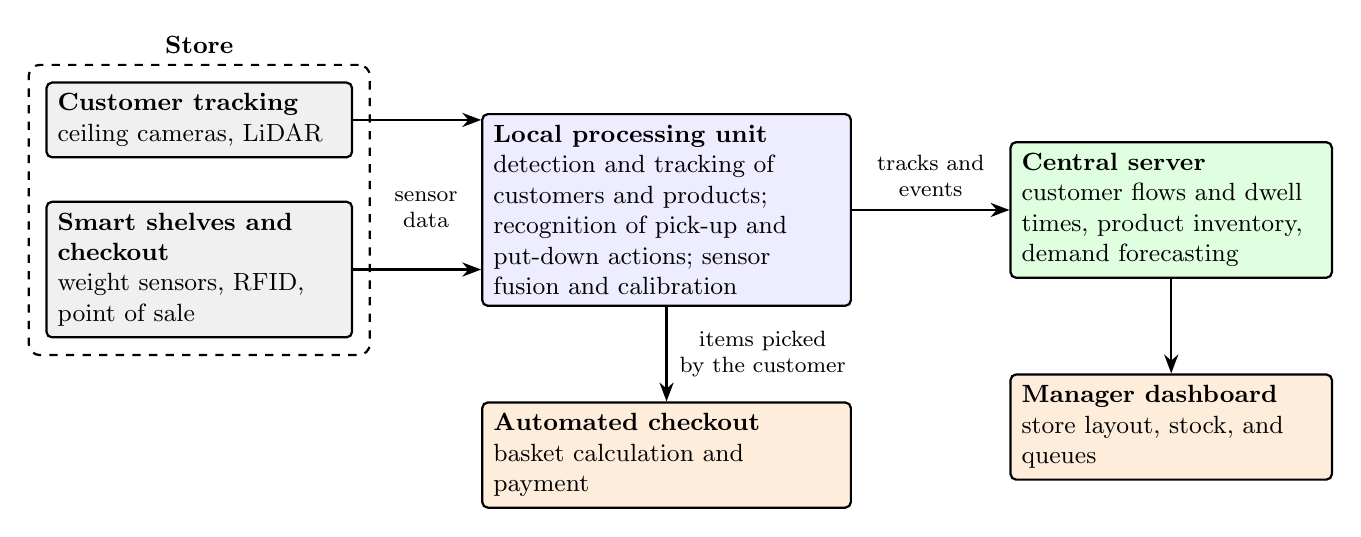
\begin{tikzpicture}[
  font=\small,
  sen/.style={draw, thick, rounded corners=2pt, fill=gray!12, align=flush left, text width=36mm, inner sep=4pt},
  loc/.style={draw, thick, rounded corners=2pt, fill=blue!7, align=flush left, text width=44mm, inner sep=4pt},
  srv/.style={draw, thick, rounded corners=2pt, fill=green!12, align=flush left, text width=38mm, inner sep=4pt},
  res/.style={draw, thick, rounded corners=2pt, fill=orange!14, align=flush left, inner sep=4pt},
  grp/.style={draw, thick, dashed, rounded corners=4pt, inner sep=6pt},
  arr/.style={-{Stealth[length=2.4mm]}, thick},
  lab/.style={font=\footnotesize, fill=white, inner sep=1.5pt, align=center}]
\node[sen] (cus) at (0,0.95) {\textbf{Customer tracking}\\ ceiling cameras, LiDAR};
\node[sen] (shelf) at (0,-0.95) {\textbf{Smart shelves and checkout}\\ weight sensors, RFID, point of sale};
\node[grp, fit=(cus)(shelf), label={[font=\small\bfseries]above:Store}] (env) {};
\node[loc, right=14mm of env] (loc) {\textbf{Local processing unit}\\ detection and tracking of customers
  and products; recognition of pick-up and put-down actions; sensor fusion and calibration};
\node[srv, right=20mm of loc] (srv) {\textbf{Central server}\\ customer flows and dwell times,
  product inventory, demand forecasting};
\node[res, text width=44mm, anchor=north] (chk) at ($(loc.south)+(0,-1.2)$) {\textbf{Automated checkout}\\
  basket calculation and payment};
\node[res, text width=38mm, anchor=north] (dash) at ($(srv.south)+(0,-1.2)$) {\textbf{Manager dashboard}\\
  store layout, stock, and queues};
\draw[arr] (cus.east) -- (loc.west |- cus.east);
\draw[arr] (shelf.east) -- (loc.west |- shelf.east);
\node[lab] at ($(env.east)!0.5!(loc.west)$) {sensor\\ data};
\draw[arr] (loc) -- node[lab, above=1mm] {tracks and\\ events} (srv);
\draw[arr] (loc) -- node[lab, right=1mm] {items picked\\ by the customer} (chk);
\draw[arr] (srv) -- (dash);
\end{tikzpicture}
\end{document}
